\documentclass[%
 reprint,
%superscriptaddress,
%groupedaddress,
%unsortedaddress,
%runinaddress,
%frontmatterverbose, 
%preprint,
%preprintnumbers,
%nofootinbib,
%nobibnotes,
%bibnotes,
 amsmath,amssymb,
 aps,
%pra,
%prb,
%rmp,
%prstab,
%prstper,
%floatfix,
]{revtex4-2}
\usepackage{multirow}
\usepackage{graphicx}% Include figure files
\usepackage{dcolumn}% Align table columns on decimal point
\usepackage{bm}% bold math
%\usepackage{hyperref}% add hypertext capabilities
%\usepackage[mathlines]{lineno}% Enable numbering of text and display math
%\linenumbers\relax % Commence numbering lines

%\usepackage[showframe,%Uncomment any one of the following lines to test 
%%scale=0.7, marginratio={1:1, 2:3}, ignoreall,% default settings
%%text={7in,10in},centering,
%%margin=1.5in,
%%total={6.5in,8.75in}, top=1.2in, left=0.9in, includefoot,
%%height=10in,a5paper,hmargin={3cm,0.8in},
%]{geometry}
\usepackage[utf8x]{inputenc} % Включаем поддержку UTF8  
\usepackage[russian]{babel}  % Включаем пакет для поддержки русского языка 
\usepackage[normalem]{ulem}  % для зачекивания текста

\usepackage[noend]{algorithmic}
\def\algorithmicrequire{\textbf{Вход:}}
\def\algorithmicensure{\textbf{Выход:}}
\def\algorithmicif{\textbf{если}}
\def\algorithmicthen{\textbf{то}}
\def\algorithmicelse{\textbf{иначе}}
\def\algorithmicelsif{\textbf{иначе если}}
\def\algorithmicfor{\textbf{для}}
\def\algorithmicforall{\textbf{для всех}}
\def\algorithmicdo{}
\def\algorithmicwhile{\textbf{пока}}
\def\algorithmicrepeat{\textbf{повторять}}
\def\algorithmicuntil{\textbf{пока}}
\def\algorithmicloop{\textbf{цикл}}
% переопределение стиля комментариев
\def\algorithmiccomment#1{\quad// {\sl #1}}

\usepackage{caption}
\usepackage{subcaption}
\usepackage{multirow}
\usepackage[table,xcdraw]{xcolor}
\begin{document}



\title{Лабораторная работа 2.2-2.3\\Изучение спектров атома водорода и молекулы йода}% Force line breaks with \\



\author{Батарин Егор Владиславович}
\affiliation{%
 Студент 3 курса РТ\\
}%

\collaboration{Московский физико-технический институт}%\noaffiliation

\date{12 сентября 2021 г.}% It is always \today, today,
             %  but any date may be explicitly specified
             

\begin{abstract}
В работе исследуются: а) сериальные закономерности в оптическом спектре водорода; б) спектр поглощения паров йода в видимой области.
\begin{description}
\item[Оборудование]
Спектрометр УМ-2, ртутная и неоновая лампы (для калибровки), водородная лампа, кристаллы йода.
\end{description}
\end{abstract}

%\keywords{Suggested keywords}%Use showkeys class option if keyword
                              %display desired
\maketitle

%\tableofcontents

\section{Теоретическая часть.}
\subsection{Основные эффекты лабы.}
В работе исследуется спектр серии Бальмера водорода и электронно-колебательный спектр йода с помощью спектрометра-монохроматора УМ-2.

 На первом рисунке показаны 0 и 1 серии Деландра, их наложение, наблюдаемое через спектрометр, и положения 1,2 и 3, соотвествующие энергиям $h\nu_{1,0},h\nu_{1,5}$ и $h\nu_\text{гр}$. В монохроматоре спектр поглощения йода наблюдается как набор темных полос, перекрывающих непрерывный спектр, начинающийся с красного цвета.

 На втором рисунке изображены линии $H_\alpha, H_\beta, H_\gamma, H_\delta$. Все линии, кроме последней, хорошо видны в спектрометре ($H_\delta$-линию обнаружить не удалось).
\begin{figure}[]
	\begin{subfigure}{0.3\textwidth}
		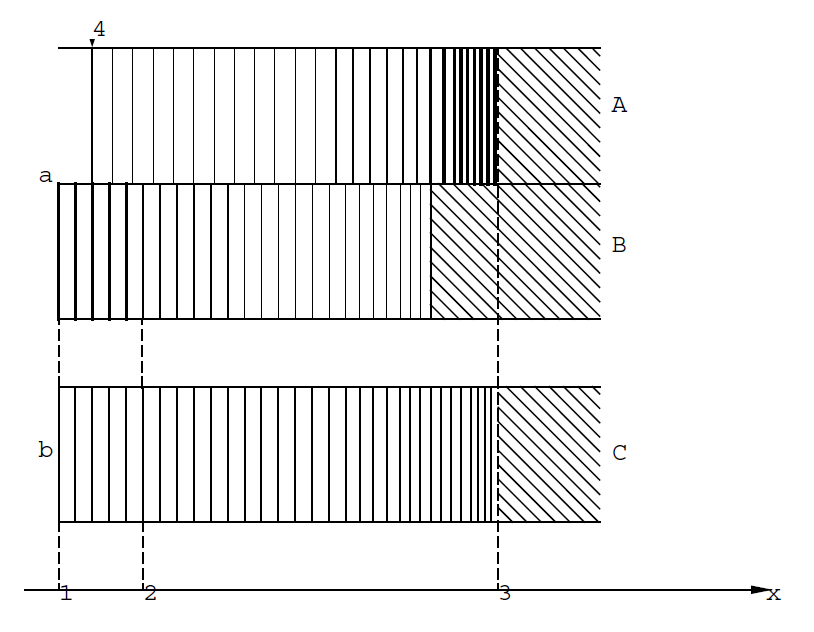
\includegraphics[scale=0.3]{1.png}
		\caption{Йод}
	\end{subfigure}
	\begin{subfigure}{0.3\textwidth}
		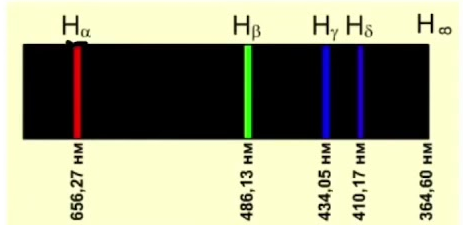
\includegraphics[scale=0.3]{2.png}
		\caption{Водород}
	\end{subfigure}
\end{figure}
\subsection{Введение в основные теоретические вещи лабы.}

В случае водорода уравнение Шредингера может быть решено точно. Его проквантованная энергия выражается формулой:
\begin{equation}
E_n= -\frac{2\pi^2m_ee^4Z^2}{h^2}\frac{1}{n^2}
\end{equation}
Из этой формулы с помощью постоянной Ридберга $R$ можно получить выражение для длин волн:
\begin{equation}
\frac{1}{\lambda_{mn}} = RZ^2\left(\frac{1}{n^2} - \frac{1}{m^2} \right)
\end{equation}
При $n=2$ получаем серию Бальмера. При этом $m=3,4,5,6$ соответсвует $H_\alpha, H_\beta, H_\gamma, H_\delta$.

Для йода картина усложняется, так как уравнение Шредингера допускает для этой молекулы более сложные состояния, включающие, помимо стандартных электронных орбиталий, колебательные движения и вращение. Можно показать, что оценка для вклада энергий имеет вид:
 \begin{equation}
 \omega_\text{эл}:\omega_\text{колеб}:\omega_\text{вращ} \approx 1 :10^{-3}:10^{-6}
 \end{equation}
Как видно из оценки $(3)$, вклад вращательного движения очень мал - именно поэтому он не учитывается в лабораторной работе. 
\section{Экспериментальная установка и методика}

Спектральный прибор по своей сути представляет из себя призму с большой дисперсией, которая раскладывает в спектр излучение от изучаемого объекта. Поворачивая призму с помощью специального барабана, можно добиться попадания нужного участка спектра в поле зрения.

В начале работы происходит калибровка монохроматора по излучению неона и ртути. Значения длин волн каждого атома, соответсвующие тем или иным положениям барабана, приведены на графике.

\begin{figure*}
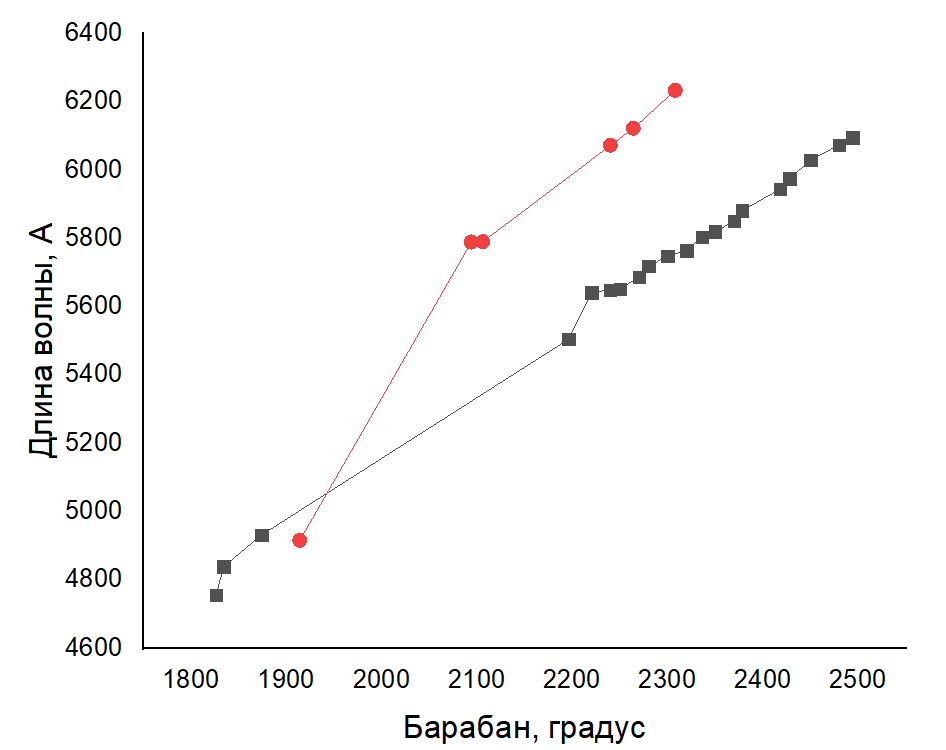
\includegraphics[scale = 0.7]{3.png}
\end{figure*}

Если отбросить некоторые точки этих графиков, то они будут очень хорошо аппроксимироваться прямой линией. По полученным линейным зависимостям будут определены соответствующие длины волн, которые будут сравниваться с эталонными.

\section{Основные результаты и их обсуждение}



\begin{table*}[]
	\begin{tabular}{|l|l|l|l|l|l|}
		\hline
		\multicolumn{6}{|c|}{{\color[HTML]{FF0000} Вычисление   длин волн $\alpha$,$\beta$,$\gamma$}}                                                                                                                           \\ \hline
		&                                                 & \multicolumn{2}{c|}{Аппроксимации, А}                      &                              &                                 \\ \cline{2-6} 
		\multirow{-2}{*}{}  & Градус барабана                                 & Неон                        & Ртуть                        & \multicolumn{2}{c|}{Длина волны(эталон), А}                    \\ \hline
		& 2440                                            & 6003.6                      & 6524                         & \multicolumn{2}{c|}{6562.8}                                    \\ \cline{2-6} 
		\multirow{-2}{*}{$\alphaб \beta$} & 1438                                            & 4059.7                      & 4419.8                       & \multicolumn{2}{c|}{4861.3}                                    \\ \hline
		$\gamma$                   & 794                                             & 2810.4                      & 3067.4                       & \multicolumn{2}{c|}{4340.3}                                    \\ \hline
		&                                                 & \multicolumn{2}{c|}{Погрешности, А}                        &                              &                                 \\ \hline
		&                                                 & Неон                        & Ртуть                        &                              &                                 \\ \hline
		$\alpha$                   & 2440                                            & 141.2                       & 324.8                        &                              &                                 \\ \hline
		$\beta$                   & 1438                                            & 111.14                      & 254.7                        &                              &                                 \\ \hline
		$\gamma$                   & 794                                             & 91.82                       & 209.6                        &                              &                                 \\ \hline
		\multicolumn{6}{|c|}{{\color[HTML]{FF0000} Сериальное отношение}}                                                                                                                                   \\ \hline
		&                                                 & Неон                        & Ртуть                        & \multicolumn{2}{c|}{Эталон}                                    \\ \hline
		$\frac{\alpha}{\beta}$                 & 1.35                                            & 1.48                        & 1.48                         & \multicolumn{2}{c|}{1.35}                                      \\ \hline
		$\frac{\alpha}{\gamma}$                   & 1.51                                            & 2.14                        & 2.13                         & \multicolumn{2}{c|}{1.51}                                      \\ \hline
		\multicolumn{6}{|c|}{{\color[HTML]{FF0000} Измерение постоянной   Ридберга}}                                                                                                                        \\ \hline
		& Расчетное значение, м\textasciicircum{}-1       & Неон, м\textasciicircum{}-1 & Ртуть, м\textasciicircum{}-1 & \multicolumn{2}{c|}{Эталон, м\textasciicircum{}-1}             \\ \hline
		$\alpha$                   & \multicolumn{1}{c|}{}                           & 11992804                    & 11036174                     & \multicolumn{2}{c|}{10970927}                                  \\ \cline{1-1} \cline{3-6} 
		$\beta$                   & \multicolumn{1}{c|}{}                           & 13137195                    & 12066911                     & \multicolumn{2}{c|}{10971002}                                  \\ \cline{1-1} \cline{3-6} 
		$\gamma$                   & \multicolumn{1}{c|}{\multirow{-3}{*}{10967760}} & 16944110                    & 15524238                     & \multicolumn{2}{c|}{10971372}                                  \\ \hline
		\multicolumn{2}{|c|}{{\color[HTML]{FF0000} Вычисления у йода:}}       & \multicolumn{2}{c|}{{\color[HTML]{FF0000} длины волны, А}} & \multicolumn{2}{c|}{{\color[HTML]{FF0000} энергии кванта, эВ}} \\ \hline
		Номер               & \multicolumn{1}{c|}{Градус барабана}            & Неон                        & Ртуть                        & Неон                         & Ртуть                           \\ \hline
		1,0                 & 2250                                            & 5635                        & 6125                         & 2.18                         & 2.01                            \\ \hline
		1,5                 & 2168                                            & 5475.9                      & 5952.8                       & 2.25                         & 2.07                            \\ \hline
		гр                  & 1704                                            & 4575.8                      & 4978.4                       & 2.69                         & 2.47                            \\ \hline
		Номер               & \multicolumn{2}{c|}{{\color[HTML]{FF0000} Вычисление энергий йода}}           & Неон                         & Ртуть                        & $h\nu_1$, эВ                       \\ \hline
		1,0                 & \multicolumn{2}{c|}{Электронный переход}                                      & 2.18                         & 2.01                         & 0.027                           \\ \hline
		1,5                 & \multicolumn{2}{c|}{Диссоциация в осноном}                                    & 1.75                         & 1.53                         & $E_{А}$ эВ                        \\ \hline
		гр                  & \multicolumn{2}{c|}{Диссоциация в возбужденном}                               & 0.51                         & 0.46                         & 0.94                            \\ \hline
	\end{tabular}
\end{table*}

Все результаты измерений и вычислений сведены в таблицу. 

Как уже было отмечено, экспериментально не удалось обнаружить $H_\delta$ линию в спектре водорода, потому придется ограничиться лишь первыми тремя. При вычислении длин волн первых трех серий были использованы линейные аппорсимация калибровочных графиков спектров неона и ртути. Сравнивая их с эталонными значениями, видим, во-первых, что спектр ртути лучше аппроксимирует истинную зависимость длины волны от поворота барабана, во- вторых, $\gamma$ линия плохо аппроксимируется обоими спектрами. Ниже приведены погрешности аппроксимаций, полученные из погрешностей МНК.

Измерение сериального отношения и постоянной Ридберга показывают, что и в этом случае спектры неона и ртути дают прохое приближение, из-за чего результаты вычислений хорошо сходятся с эталоном только для $\alpha$ и $\beta$ линий, где и проводилась калибровка ламп.

В низу таблицы приведены измерения различных энергий для молекулы йода. Результаты вычислений верно отражают порядок полученных значений (тем не менее, нельзя достоверно ручаться про мантиссы, так как экспериментально было сложно определить, где начинается $h\nu_{1,0}$ и заканчивается $h\nu_\text{гр}$ )

\section{Заключение}

В работе были выполены соедующие задачи:

1) Исследована серия Бальмера водорода, вычислены длины волн и постоянная Ридберга

2) Исследован электронно-колебательный спектр йода, вычислены энергии перехода и диссоциации.




\end{document}